
%(BEGIN_QUESTION)
% Copyright 2011, Tony R. Kuphaldt, released under the Creative Commons Attribution License (v 1.0)
% This means you may do almost anything with this work of mine, so long as you give me proper credit

This partial P\&ID shows a pressure control system, where a controller throttles the amount of cooling water to a heat exchanger (the ``vapor cooler'') to affect the amount of pressure in a vessel filled with condensible vapors.  The more cooling water through the exchanger, the faster those vapors will condense back into liquid, decreasing pressure in the vessel:

$$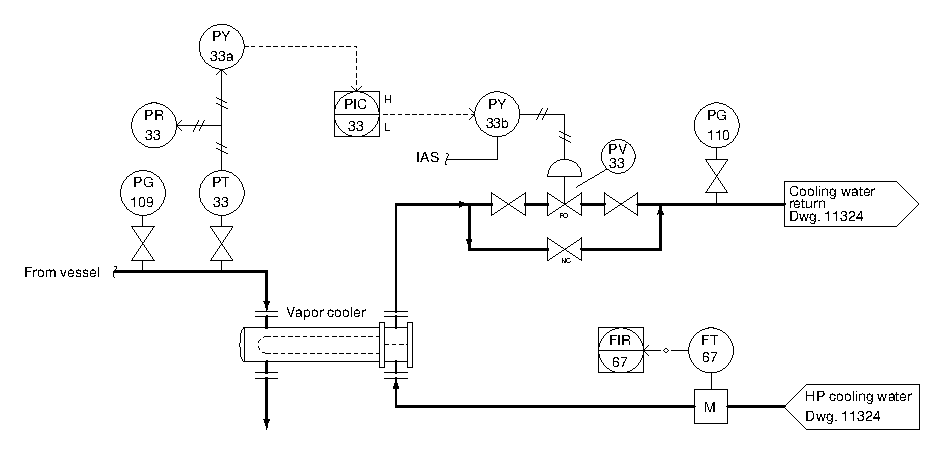
\includegraphics[width=15.5cm]{i03563x01.eps}$$

PG-109 and PR-33 both register 37 PSI of pressure, but PIC-33 registers 40 PSI of pressure (which happens to be right on setpoint).  Based on this information, some instrument technicians suggest faults to account for this discrepancy.  Analyze and explain why each proposed fault either is or is not possible:

\vskip 20pt

Pressure transmitter PT-33 has a calibration error:

\vskip 40pt

Pressure control valve PV-33 has a calibration error:

\vskip 40pt

Pressure transducer PY-33a has a calibration error:

\vskip 40pt

Pressure recorder PR-33 has a calibration error:

\vskip 40pt

Pressure controller PIC-33 has been left in manual mode:

\vskip 40pt

\filbreak

\underbar{file i03563}
%(END_QUESTION)





%(BEGIN_ANSWER)

(2 points for each correct answer)

\vskip 10pt

Pressure transmitter PT-33 has a calibration error: {\bf NO, because then the recorder's indication would not agree with the gauge's.}

\vskip 10pt

Pressure control valve PV-33 has a calibration error: {\bf NO, because it would not make any pressure instrument disagree with any other.}

\vskip 10pt

Pressure transducer PY-33a has a calibration error: {\bf YES, because this would skew the controller's reading of pressure apart from the recorder and gauge.}

\vskip 10pt

Pressure recorder PR-33 has a calibration error: {\bf NO, because then the recorder's indication would not agree with the gauge's.}

\vskip 10pt

Pressure controller PIC-33 has been left in manual mode: {\bf NO, because all the pressure instruments' indications would agree with each other.}

\vskip 10pt


%(END_ANSWER)





%(BEGIN_NOTES)

{\bf This question is intended for exams only and not worksheets!}.

%(END_NOTES)


